\cleardoublepage
\section{Anhang}
\subsection{Thekenaufbau}
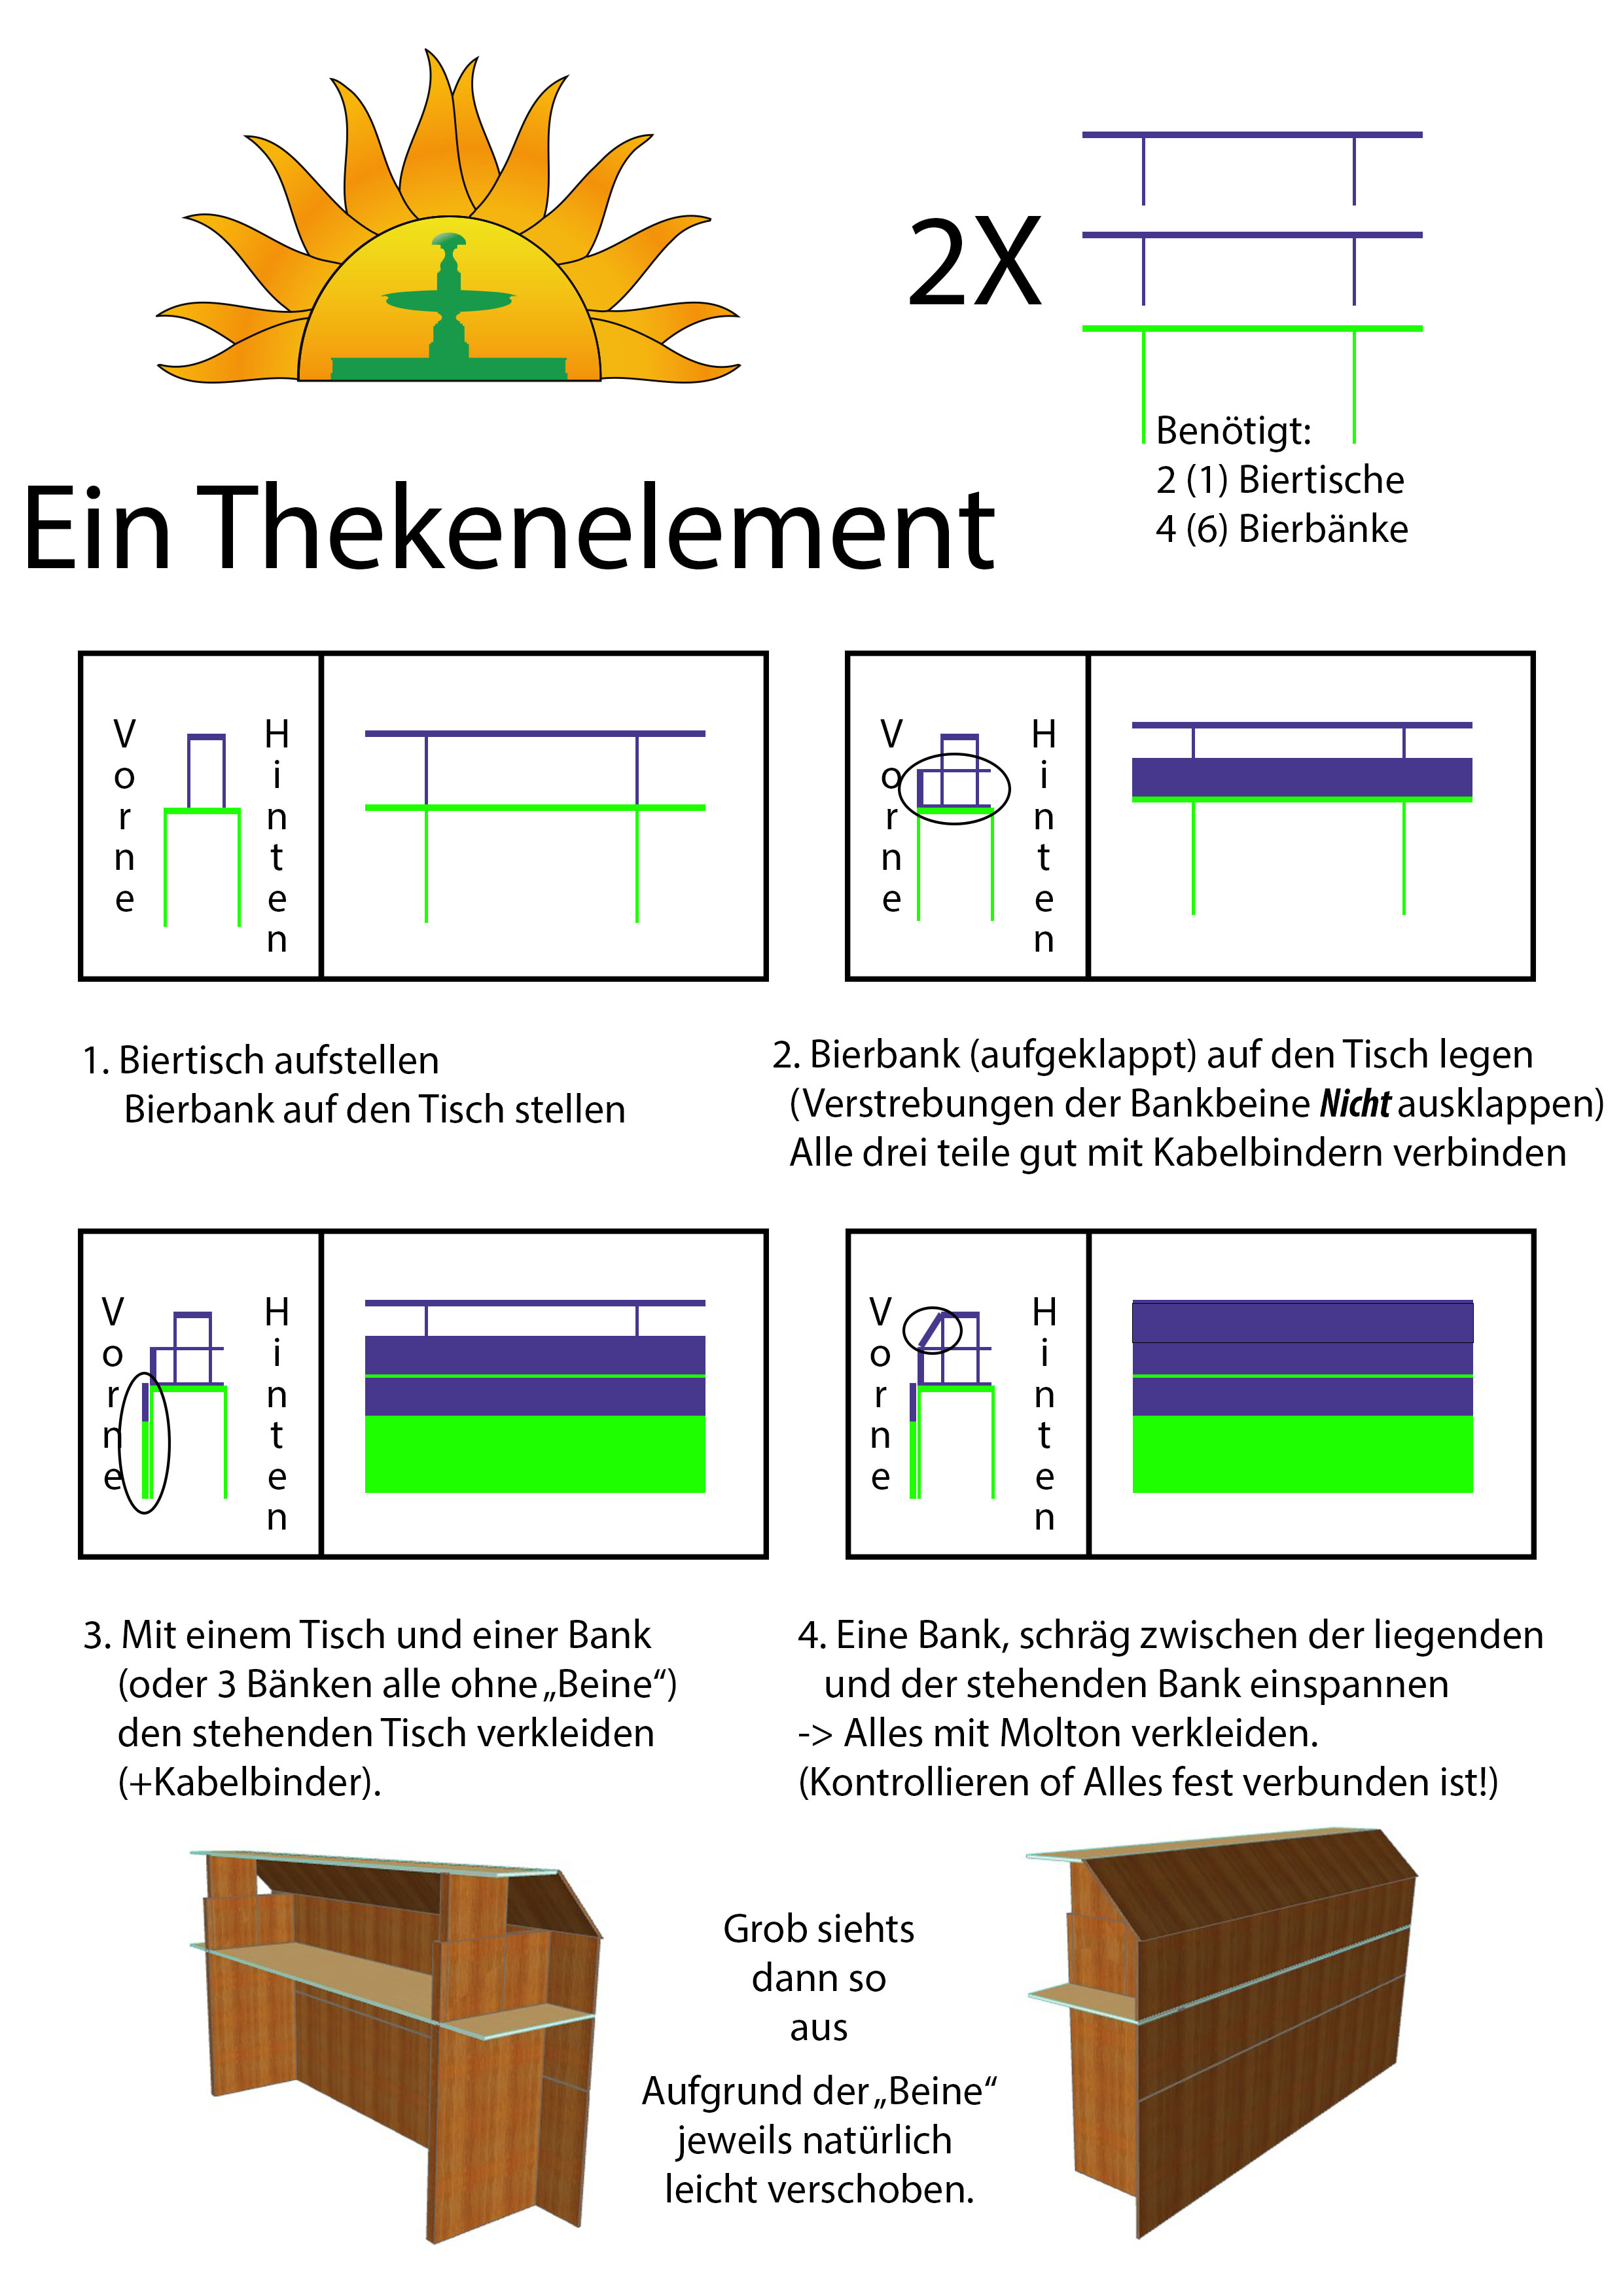
\includegraphics[width=.95\textwidth]{theke.jpg}
%\tiny{
%\begin{figure}[h]
%  \centering
%  \begin{subfigure}[t]{0.45\textwidth}
%    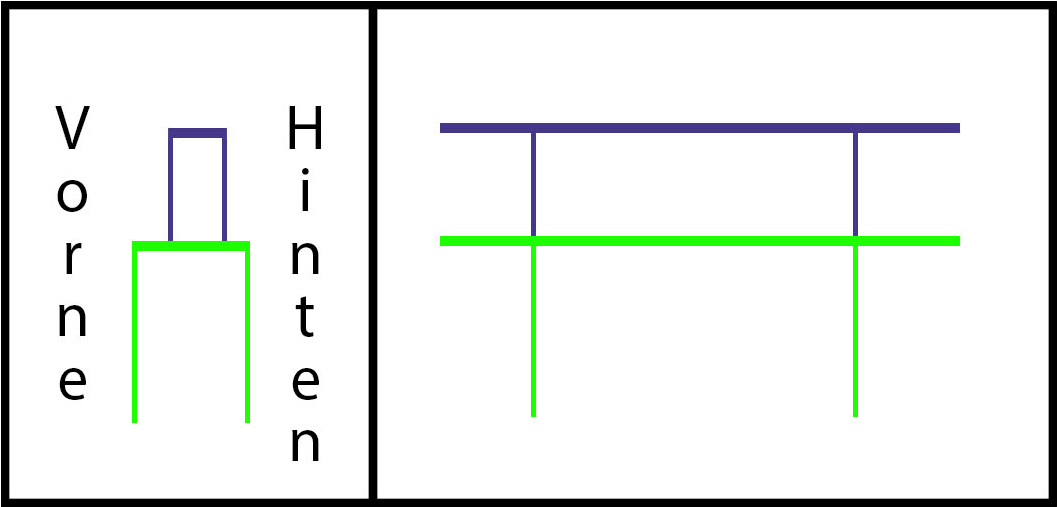
\includegraphics[width=\textwidth]{2d_1.png}
%    \caption{Einen Tisch aufstellen und eine aufgeklappte Bank darauf stellen.}
%  \end{subfigure}
%  \hfill
%  \begin{subfigure}[t]{0.45\textwidth}
%    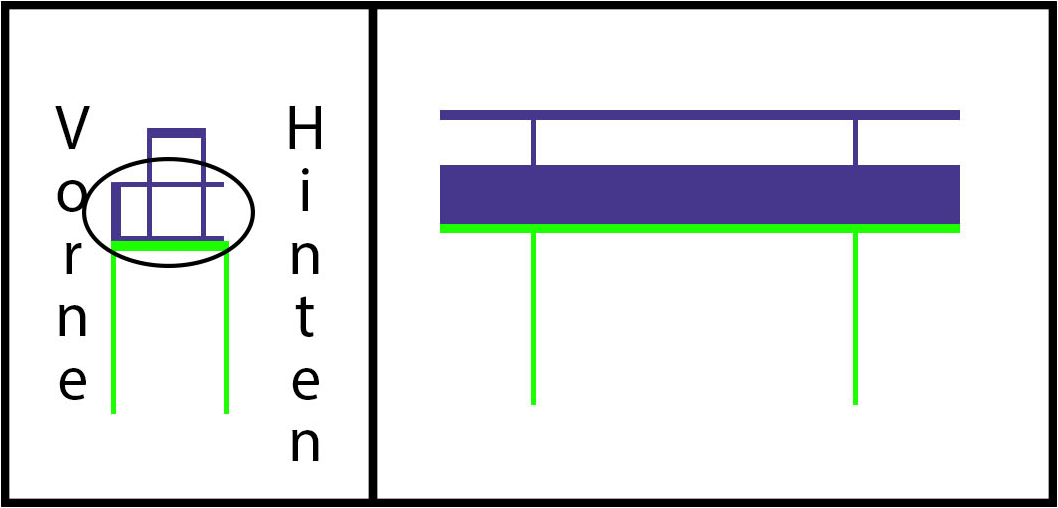
\includegraphics[width=\textwidth]{2d_2.png}
%    \caption{Eine Bank aufklappen, aber die diagonalen Arretierungen eingeklappt lassen. Die Bank senkrecht zum Tisch hinlegen und alle drei Teile mit Kabelbindern befestigen, aber noch nicht ganz festzurren.}
%  \end{subfigure}
%  \centering
%  \begin{subfigure}[t]{0.45\textwidth}
%    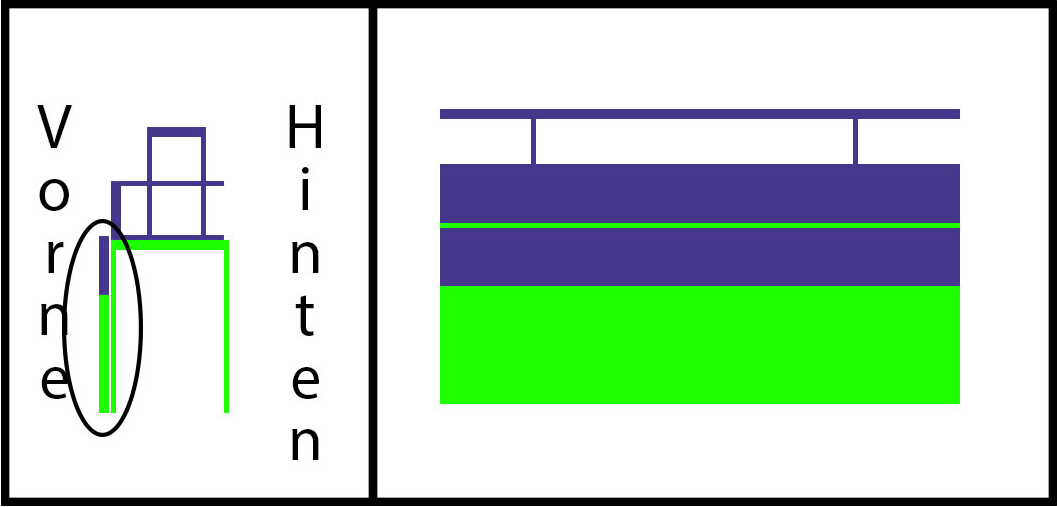
\includegraphics[width=\textwidth]{2d_3.png}
%    \caption{Die Vorderseite mit 1 Tisch und 2 Bänken, oder 3 Bänken verkleiden und mit Kabelbindern verbinden (die Beine jeweils eingeklappt lassen, sonst stehen sie innen über).}
%  \end{subfigure}
%  \hfill
%  \begin{subfigure}[t]{0.45\textwidth}
%    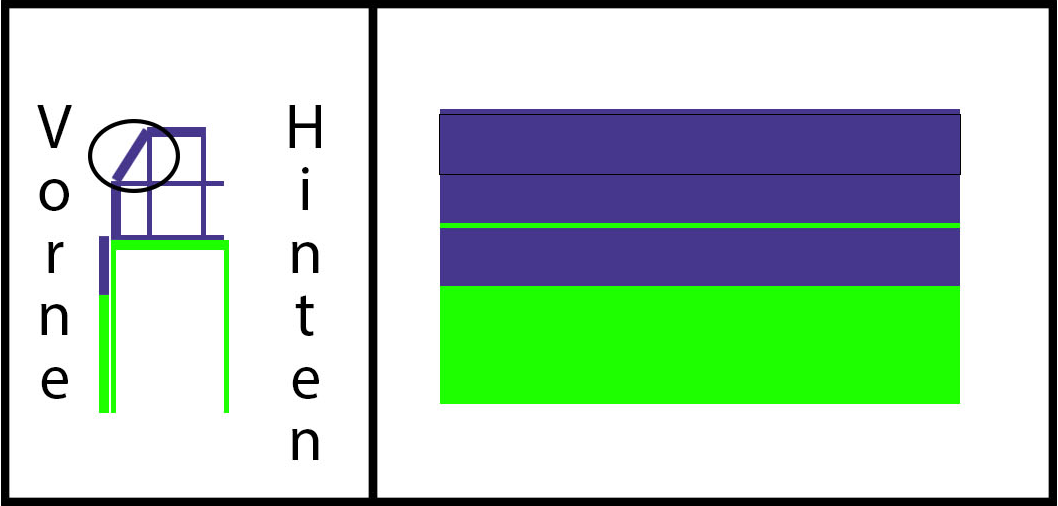
\includegraphics[width=\textwidth]{2d_4.png}
%    \caption{Eine Bank (auch ohne Beine) schräg zwischen der liegenden und der stehenden Bank einspannen und mit Kabelbindern festzurren.}
%  \end{subfigure}
%  \label{theke2d}
%\end{figure}
%\begin{figure}[h]
%  \begin{subfigure}[t]{0.45\textwidth}
%    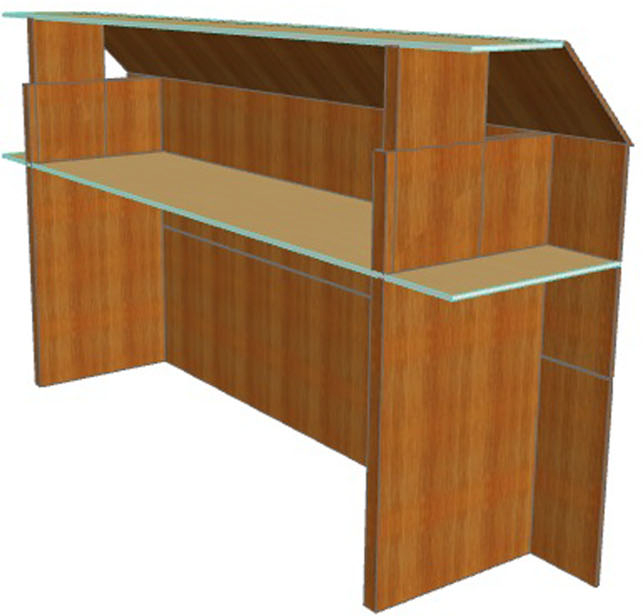
\includegraphics[width=.7\textwidth]{3d_hinten.png}
%  \end{subfigure}
%  \begin{subfigure}[t]{0.45\textwidth}
%    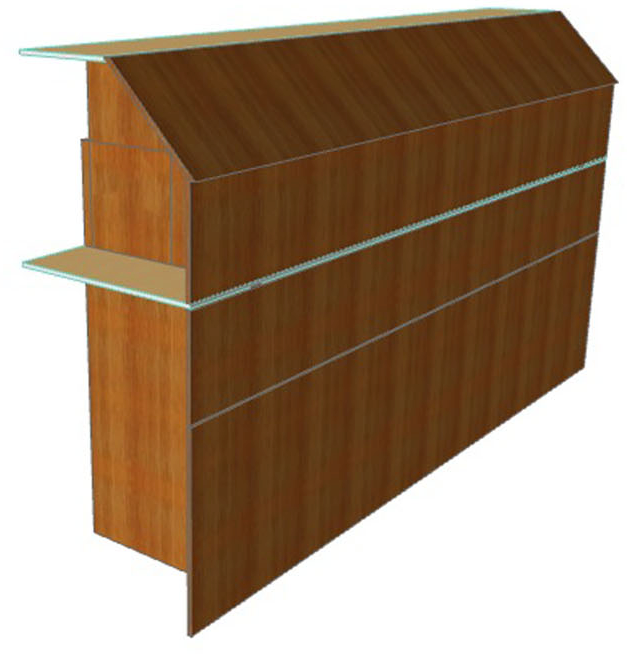
\includegraphics[width=.7\textwidth]{3d_vorne.png}
%  \end{subfigure}
%  \label{theke3d}
%\end{figure}
%}
\cleardoublepage
%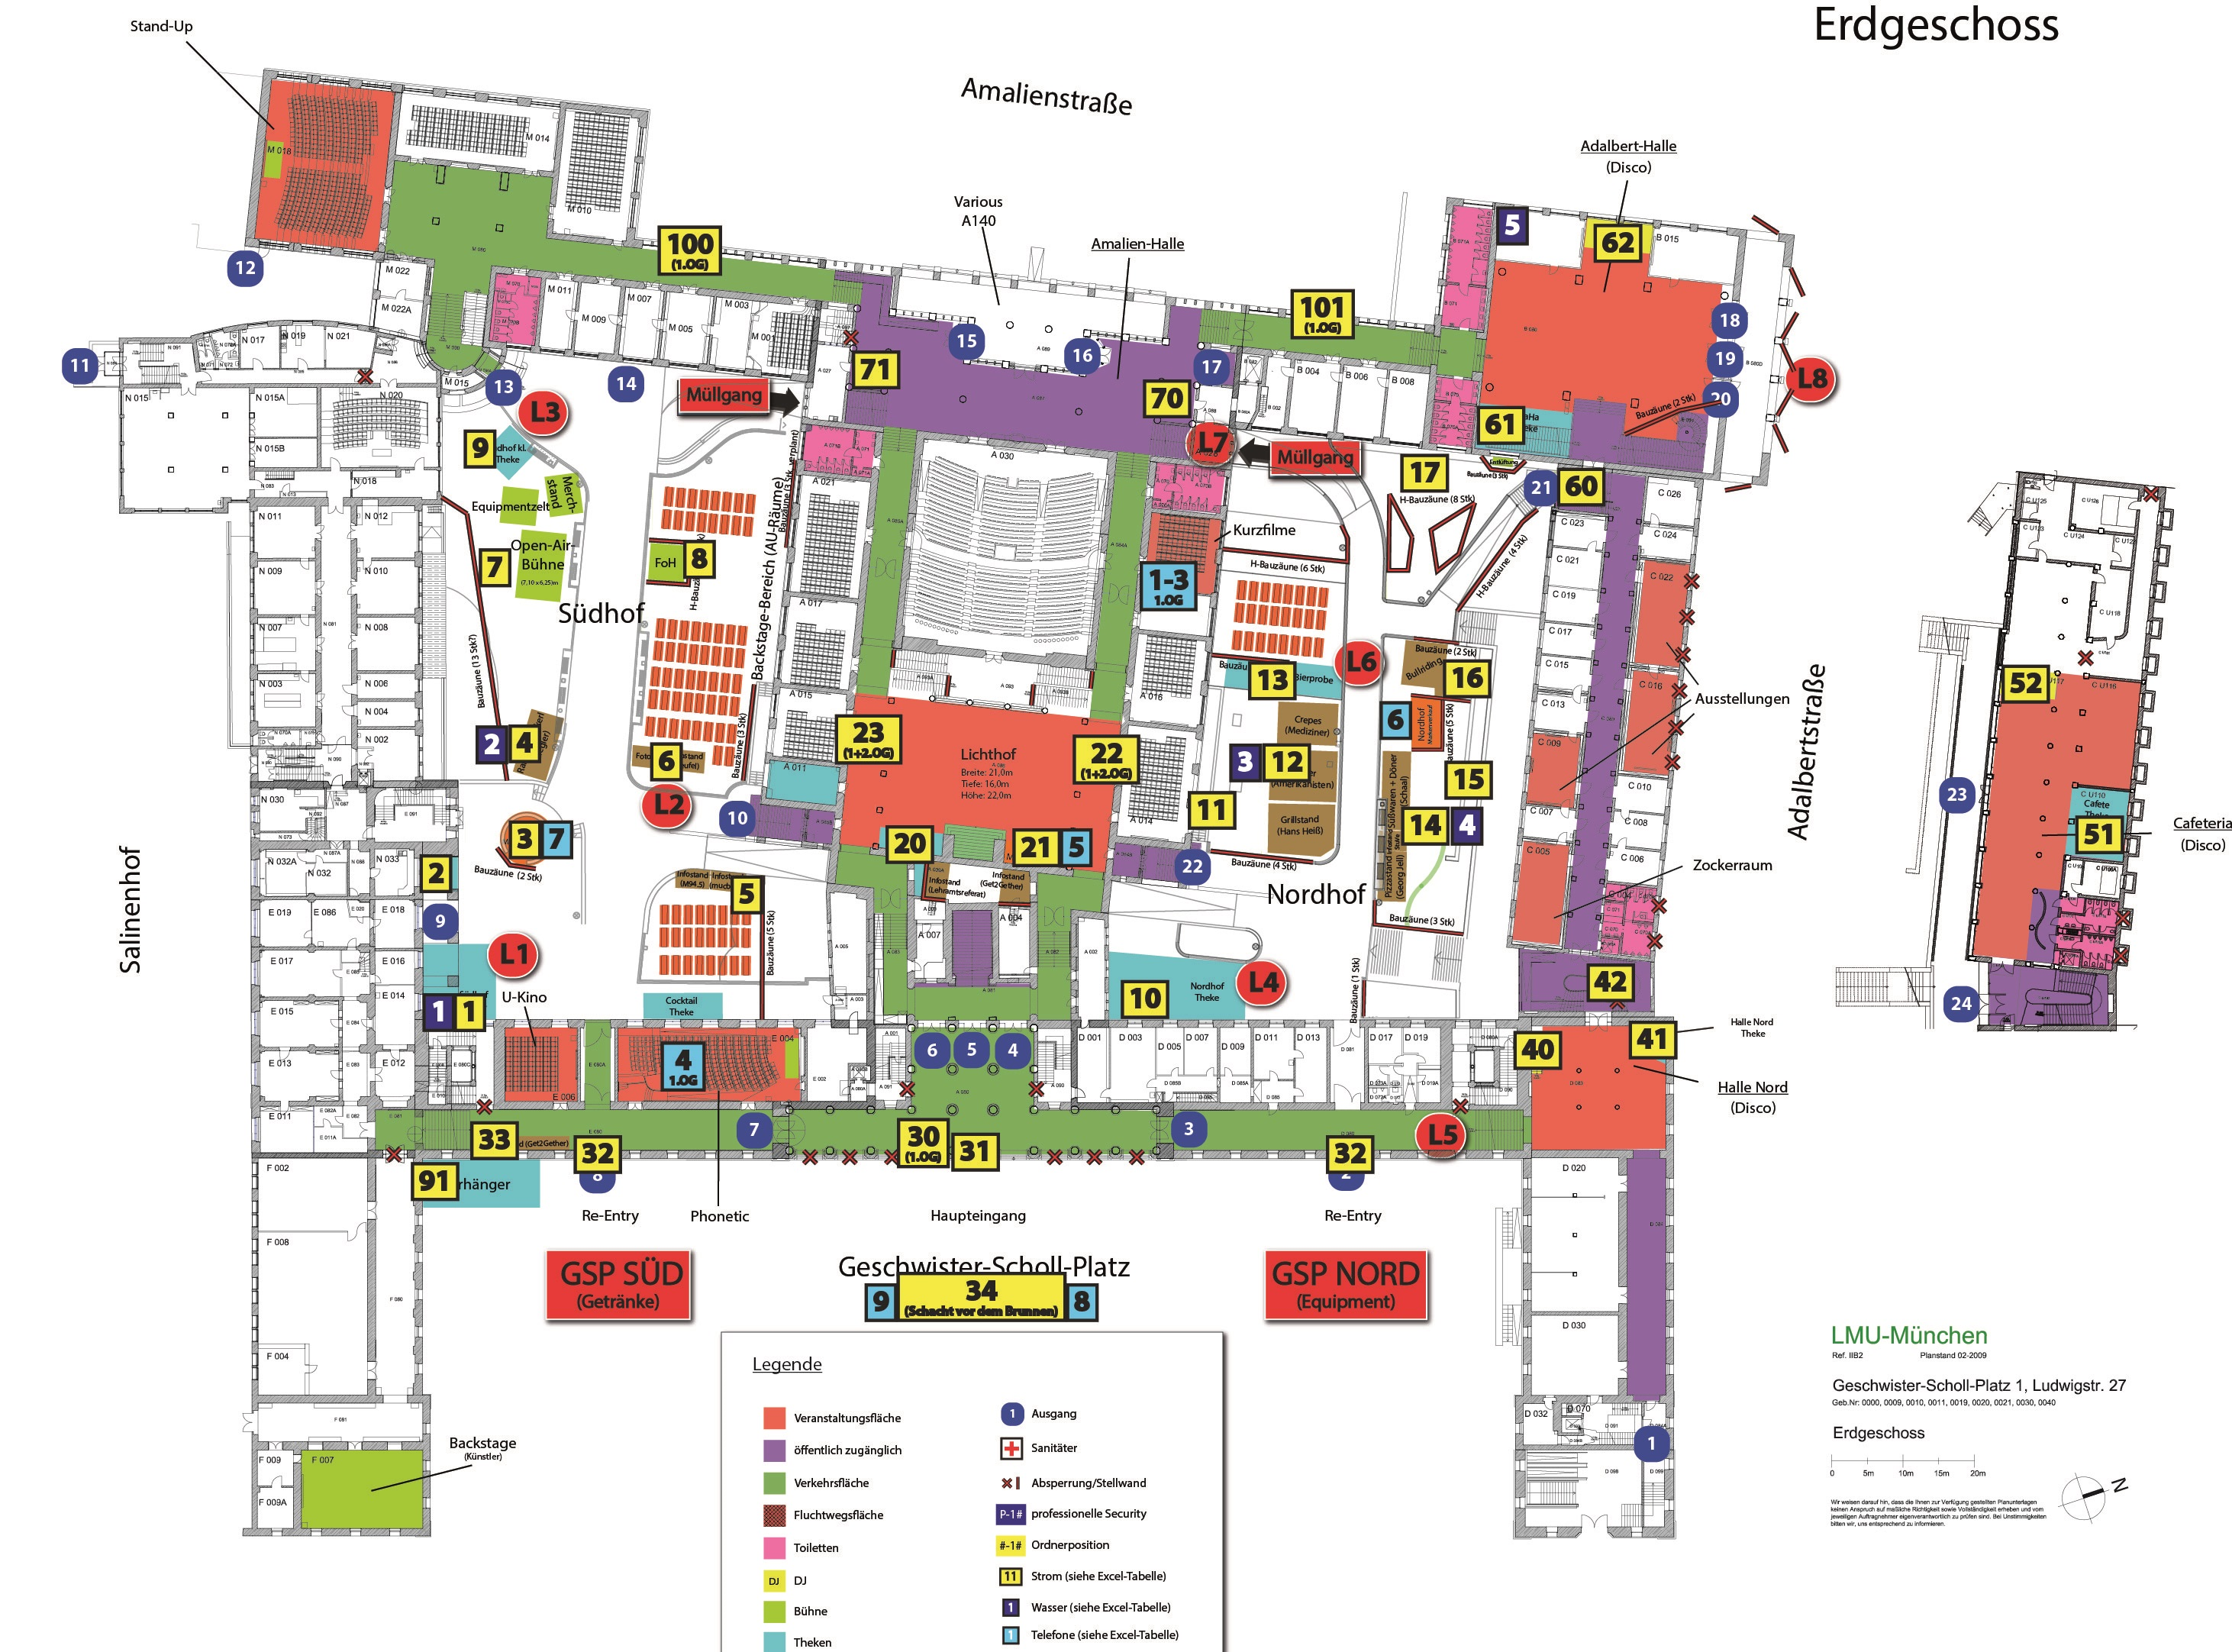
\includegraphics[height=\textwidth, angle=270]{plan.jpg}
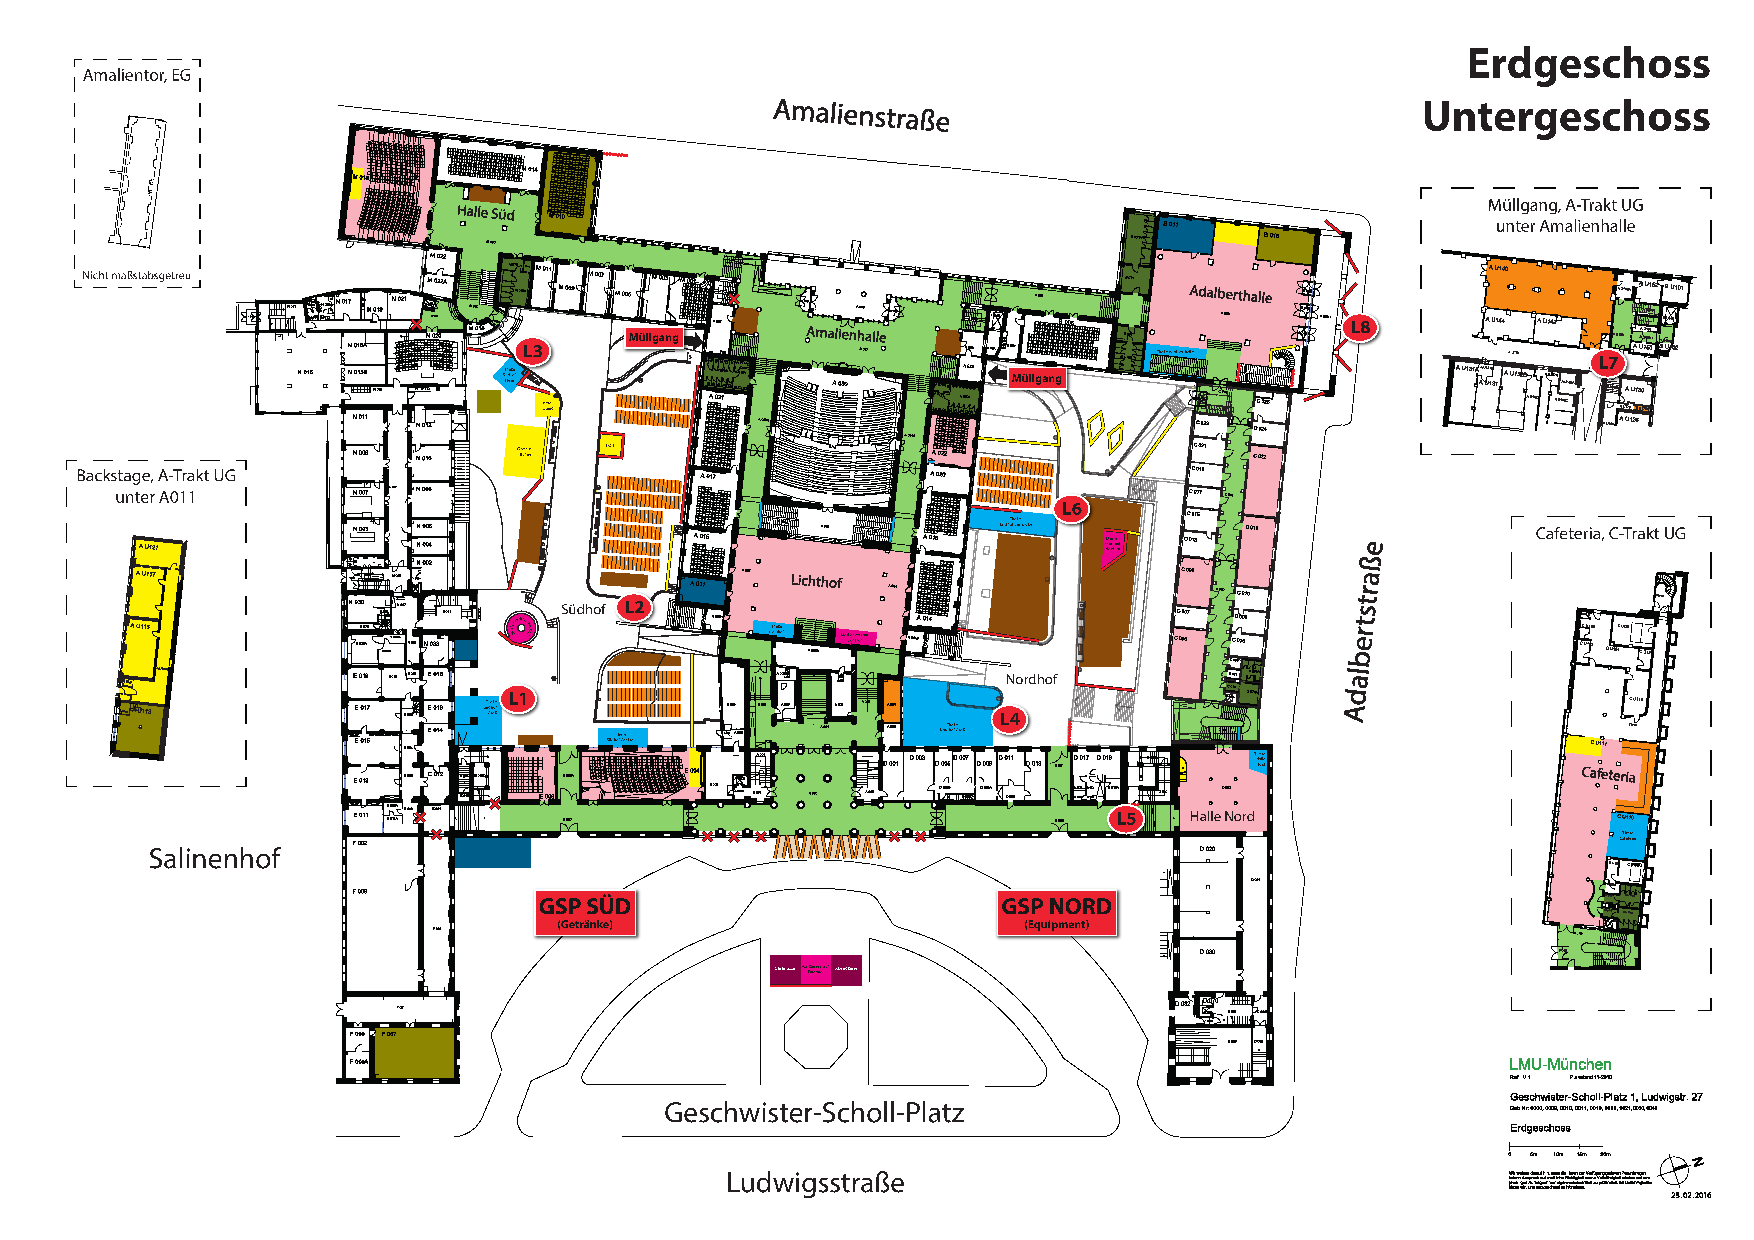
\includepdf[angle=90, pages=-]{Festplan_2016.pdf}
